%CONFIGURACIÓN DEL DOCUMENTO Y HOJA

\documentclass[11pt,letterpaper]{article}
\setlength{\parindent}{0em}                  %DISTANCIA SANGRÍA
\setlength{\parskip}{0.5em}                  %DISTANCIA ENTRE PÁRRAFOS
\textwidth 6.5in
\textheight 9.in
\oddsidemargin 0in
\headheight 0in

%PAQUETES DEL TEMPLATE

\usepackage{fancybox}
\usepackage[utf8]{inputenc}
\usepackage{epsfig,graphicx}
\usepackage{multicol,pst-plot}
\usepackage{pstricks}
\usepackage{amsmath}
\usepackage{amsfonts}
\usepackage{amssymb}
\usepackage{eucal}
\usepackage[left=2cm,right=2cm,top=2cm,bottom=2cm]{geometry}
\usepackage{txfonts}
\usepackage[spanish]{babel}
\usepackage[colorlinks]{hyperref}
\usepackage{cancel}
\usepackage{caption}
\usepackage{float}
\usepackage{upgreek}
\usepackage{gensymb}
\usepackage{subfigure}
\usepackage{siunitx}
\usepackage{color}
\usepackage{tikz}
\usepackage{listings}
\usepackage{minted}
\usepackage{mdframed}
\usepackage[
backend=bibtex,
style=ieee,
sorting=none
]{biblatex}
\addbibresource{biblio.bib}
\usepackage{multicol}
\usepackage{stackrel}

%DEFINICIÓN DE COLORES EXTRAS

\definecolor{codegreen}{rgb}{0,0.6,0}
\definecolor{codegray}{rgb}{0.5,0.5,0.5}
\definecolor{backcolour}{rgb}{0.95,0.95,0.95}
\hypersetup{colorlinks=true,linkcolor=codegreen,citecolor=blue,filecolor=blue,urlcolor=magenta,}

%CONFIGURACIÓN DE LSTLISTINGS PARA CÓDIGOS

\lstset{ %
language=python,                % choose the language of the code
basicstyle=\footnotesize,       % the size of the fonts that are used for the code
numbers=left,                   % where to put the line-numbers
numberstyle=\footnotesize,      % the size of the fonts that are used for the line-numbers
stepnumber=1,                   % the step between two line-numbers. If it is 1 each line will be numbered
numbersep=5pt,                  % how far the line-numbers are from the code
backgroundcolor=\color{white},  % choose the background color. You must add \usepackage{color}
showspaces=false,               % show spaces adding particular underscores
showstringspaces=false,         % underline spaces within strings
showtabs=false,                 % show tabs within strings adding particular underscores
frame=single,                   % adds a frame around the code
tabsize=2,                      % sets default tabsize to 2 spaces
captionpos=b,                   % sets the caption-position to bottom
breaklines=true,                % sets automatic line breaking
breakatwhitespace=false,        % sets if automatic breaks should only happen at whitespace
escapeinside={\%*}{*)}          % if you want to add a comment within your code
}
\lstdefinestyle{mystyle}{
	backgroundcolor=\color{backcolour},
	commentstyle=\color{red},
	keywordstyle=\bfseries\color{magenta},
	numberstyle=\tiny\color{codegray},
	stringstyle=\color{codegreen},
	basicstyle=\footnotesize\ttfamily,
	identifierstyle=\color{blue},
	breakatwhitespace=false,
	breaklines=true,
	captionpos=b,
	keepspaces=true,
	numbers=left,
	numbersep=5pt,
	showspaces=false,
	showstringspaces=false,
	showtabs=false,
	tabsize=2
}

\lstset{style=mystyle}

%CONFIGURACIÓN DE MINTED PARA CÓDIGOS

\usemintedstyle{vs}

%DEFINICIÓN DE COMANDOS EXTRAS

\pagestyle{empty}
\newcommand{\units}[1]{\left[ #1 \right]}          %CORCHETES PARA UNIDADES
\newcommand{\abs}[1]{\left|#1\right|}              %OPERADOR VALOR ABSOLUTO INTEGRALES

%COMIENZA EL DOCUMENTO

\begin{document}

%CONFIGURACIÓN DEL ENCABEZADO

\usetikzlibrary{positioning}
\tikzset{every picture/.style={line width=0.75pt}}
\pagestyle{plain}
\begin{flushleft}
Ingeniería de la Salud \hfill Bioinformática\\
Escuela Técnica Superior de Ingeniería Informática\\
\underline{Universidad de Málaga}
\end{flushleft}

\begin{flushright}\vspace{-5mm}

\includegraphics[height=1.5cm]{escudo.jpg}
\end{flushright}

\begin{center}\vspace{-1cm}
\textbf{\large Práctica 4. Plegado de cadenas de ARN.}\\   %TITULO
Arrabalí Cañete, Carmen Lucía\\                         %NOMBRE
\end{center}
\rule{\linewidth}{0.1mm}

%DESDE AQUÍ SE ESCRIBE TODO EL CONTENIDO

\section{Introducción y objetivos}
El algoritmo de Nussinov es un algoritmo de predicción de la estructura del ácido nucleico utilizado en biología computacional para predecir el plegamiento de una molécula de ARN que hace uso de principios de programación dinámica.  

Fue uno de los primeros algoritmos desarrollados para la predicción de estructuras de ARN, ya que la combinatoria de ARN puede ser bastante costosa y complicada. 

\subsection{Contexto Biológico del problema}
La función principal del ARN es, básicamente, servir como medio entre la información que aporta el ADN y la proteína a la que le llega toda esta información,para realizar la síntesis proteica, además, gracias a la acción del ARN la síntesis proteica se produce en su justa medida. Esta función se considera un proceso de traducción entre el ADN y la proteína. 

\subsection{ARN y Nussinov}
Se puede definir el ARN como una secuencia $S$, que está formada por cuatro bases nitrogenadas, $S \in \left\{C, G, A, U\right\}$. Estas cuatro bases vienen en pares y se combinan de la siguiente manera $A \leftrightarrow U$ y $G \leftrightarrow C$.

Estos son los pares de bases mas fuertes o estables, llamados pares de bases de Watson-Crick, pero también se tiene el acoplamiento de pares menos estables, conocidos como pares de bases de Wobble, los cuales son $G \leftrightarrow U$.

Por lo tanto, la predicción de la estructura secundaria del ARN sería que dada una molécula de ARN $S = s_{1}, s_{2}, ..., s_{n}$, donde cada nucleótido $s_{i} \in \left\{C, G, A, U\right\}$, para $1 \leqslant i \leqslant n$, se tiene que encontrar un conjunto de pares de bases compatibles $P \subset \left\{(i, j) | 1 \leqslant i < j \leqslant n\right\}$ de cardinalidad máxima, respetando cualquier restricción estructural que pueda existir, en este caso se tiene que tener en cuenta la compatibilidad de los pares de bases que se explicó con anterioridad.

También hay que tener en cuenta las restricciones estructurales:

\begin{itemize}
	\item \textbf{Sin Pseudoknots}: P no se cruza. Para cualquier $(i, j),(i^{'}, j^{'}) \in  P$, no puede ocurrir que $i< i^{'} < j < j^{'}$.
	\item \textbf{Tamaño del bucle o Loop Size}: Para cualquier $(i, j) \in P, j - i > L $, donde  $L$ es el tamaño mínimo del bucle del tallo (también conocido como horquilla o hairpin-loop).
\end{itemize}

\subsection{Ecuación de Bellman}

\begin{figure}[H]
	\centering
	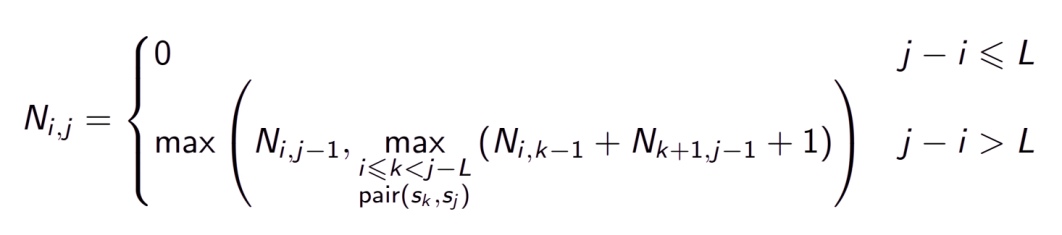
\includegraphics[width=0.65\textwidth]{bellman.png}
	\caption{Ecuación de Bellman}
	\label{fig:bellman}
\end{figure}

\section{Configuración del equipo}
Se ha realizado la implementación en un equipo con un sistema operativo Windows 10 Home 64 bits, con un procesador Intel$($R$)$ Core $($TM$)$ i7-6500U CPU $@$ 2.50GHz 2.59 GHz $($4 CPUs$)$ y un disco SSD de 480GB y 12GB de RAM. La versión Java corresponde a la número 17.

\section{Implemetación}

En el primer método de la implementación, \textit{protected String \_run} de la clase \textit{Nussinov} (ver apartado ~\ref{ch:31}) recibe como parámetros un String con la cadena de ARN y el tamaño mínimo de plegado, en la realidad suele estar entre 4 y 8, pero el algoritmo puede aceptar cualquier valor. Se encarga de implementar la ecuación de Bellman (véase figura~\ref{fig:bellman}) y de devolver la secuencia de ARN plegada, es decir, se encarga de calcular la matriz de decisiones $D$ y hacer una llamada al segundo método \textit{private String reconstructSolution} (ver apartado ~\ref{ch:32}) de la misma clase, el cual se encarga de, recibiendo como parámetros la matriz de decisiones D y los índices i y j desde los que se debe reconstruir la solución, devolver la secuencia de ARN como un String haciendo uso de la notación Dot-Backet.

En el primer bucle, línea 7 del primer método (ver apartado ~\ref{ch:31}) se encarga de comprobar si los nucleótidos que se estudian son compatibles entre sí en función de las restricciones comentadas anteriormente.

Los siguientes dos bucles, línea 13, se encargan del caso base de la ecuación de Bellman (véase figura~\ref{fig:bellman}), cuando $M(i,j) = 0$ si $j \leqslant i+minloopSize$.

Por último, en la línea 21, los tres bucles anidados se encargan principalmente de la segunda parte de la ecuación de Bellman (véase figura~\ref{fig:bellman}), que trata del caso general cuando $M(i,j) = max(M(i,j-1), max (M(i, k-1) + M(k+1,j-1) + 1$ donde $i \leqslant k < j-minloopSize$ y $s_{k}$ y $s_{j}$ son complementarios$))$ si $j > i+minloopSize$

\newpage
\subsection{Método \textit{protected String \_run} de la clase \textit{Nussinov}}\label{ch:31}

\begin{lstlisting}[language = java]
	protected String _run(String rnaSeq, int minLoopSize) {
		int n = rnaSeq.length();			// number of nucleotides in the sequence
		int[][] M = new int[n][n+1];		// to store costs
		int[][] D = new int[n][n];			// to store decisions
		boolean[][] B = new boolean[n][n];	// to precompute which base pairs match
		
		for (int i=0; i<n; i++) {
			for (int j=i+1; j<n; j++) {
				B[i][j] = isCompatible(rnaSeq.charAt(i), rnaSeq.charAt(j));
			}
		}	
		
		for (int i = 0; i < n; i++) {
			M[i][i] = 0;				// M(i,i-1) = 0
			for (int j = i, k = 0; (k <= minLoopSize) && (j<n); j++, k++) {
				M[i][j+1] = 0;			// M(i,j) = 0;
				D[i][j] = -1;			// -1 => unpaired
			}
		}
		
		for (int j = 0; j < n; j++) {
			for (int i = 0; i < j; i++) {
				int newJ = j+1;
				M[i][newJ] = M[i][newJ-1];				
				int bestK = -1;
				for (int k = i; k < newJ-minLoopSize-1; k++) {
					int newK = k+1;
					if (B[k][j] && M[i][newJ] < M[i][newK-1] + M[k+1][newJ-1] + 1) {
						M[i][j+1] = M[i][newK-1] + M[k+1][newJ-1] + 1 ;
						bestK = k;
					}
				}
				D[i][j] = bestK;
			}
		}
		// Hay un trozo de codigo adicional que se encarga de imprimir por pantalla
		// la matriz de decisiones.
		
		// Reconstruction of the optimal solution
		return reconstructSolution(D, 0, n-1);
	}
\end{lstlisting}

\newpage
\subsection{Método \textit{private String reconstructSolution} de la clase \textit{Nussinov}}\label{ch:32}
\begin{lstlisting}[language = java]
	private String reconstructSolution (int[][] D, int i, int j) {
		// TODO
		// returns the folding in dot-bracket notation.
		// use a recursive approach for simplicity
		String result = "";	
		if (j>i-1) {
			int k = D[i][j]; 
			if (k>-1) {
				return reconstructSolution(D,i,k-1) +"(" + reconstructSolution(D,k+1,j-1) +")";			
			}
			else {
				return reconstructSolution(D, i, j-1) + ".";
			}
		}else if(j == i){
			result = ".";
		}
		return result;
	}
	
\end{lstlisting}

\section{Resultados y Conclusiones}
Para poder analizar correctamente los resultados, el método main recibe en los argumentos de entrada, varios modos de ejecución entre los que se encuentra \textit{$-$r $<$init\_length$>$ $<$doubling$>$ $<$num\_seq$>$ $<$minlop$>$} el cual genera un archivo con secuencias de ARN aleatorias con distintas longitudes. Se generan \textit{num\_seq} secuencias de cada longitud, que empezará con \textit{init\_length} y se irá doblando tantas veces como indique el parámetro \textit{doubling}. Por último, se pasa como parámetro la separación mínima para plegar nucleótidos.

Al utilizar ese modo de ejecución, se genera un archivo con los diferentes tiempos de ejecución, el cual se llama  un archivo \textit{folding.txt}.

Por otro lado, entre los recursos aportados en el Campus Virtual se tiene un archivo llamado \textit{analyze.R} que contiene un script el cual se encarga de generar una gráfica haciendo uso del archivo .txt generado anteriormente con el modo de ejecución $-$r.

\begin{figure}[H]
	\centering
	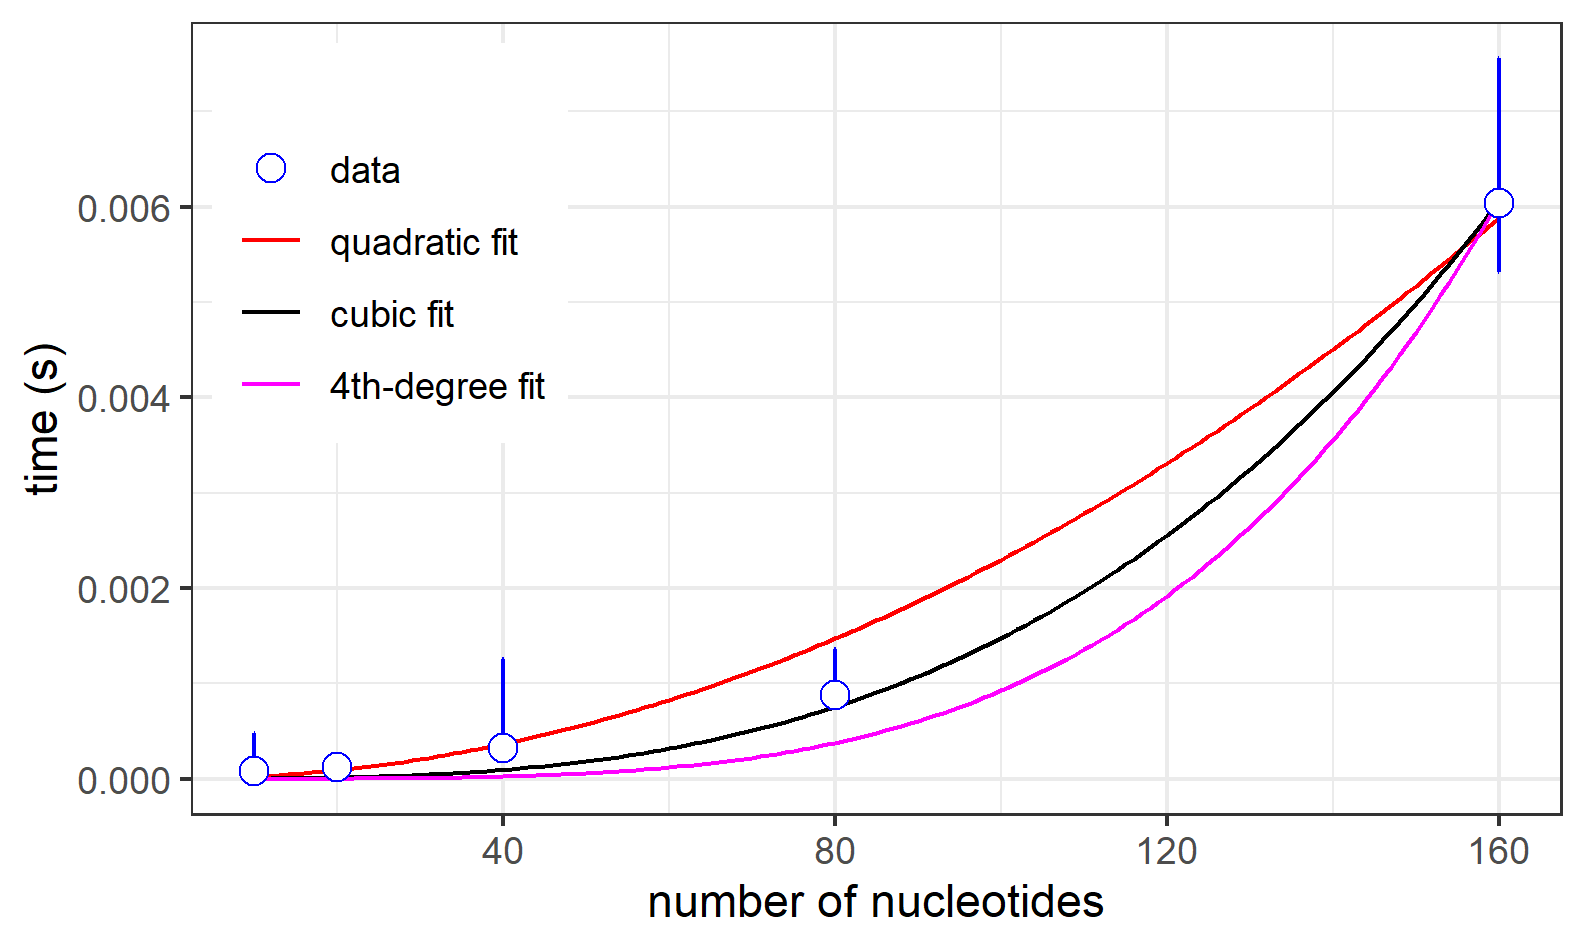
\includegraphics[width=0.65\textwidth]{folding.png}
	\caption{Resultado de la ejecución del algoritmo con los parámetros utilizados.}
	\label{fig:grafico}
\end{figure}

Para poder generar un archivo con unos datos asequibles para el algoritmo y para el equipo que se utiliza, se han dado los siguientes valores: 

\begin{multicols}{2}
	\begin{itemize}
		\item \textbf{$<$init\_length$>$}: 10
		\item \textbf{$<$doubling$>$}: 5
		\item \textbf{$<$num\_seq$>$}: 20
		\item \textbf{$<$minlop$>$}: 6
	\end{itemize}
\end{multicols}

Como se puede observar en la figura~\ref{fig:grafico}, cuanto mayor sea el número de nucleótidos de la cadena con la que se quiere obtener el plegamiento, el tiempo que tarda el algoritmo en obtener el resultado también es mayor, tanto de forma cuadrática, como cúbica, como, incluso, de cuarto grado, hasta llegar al límite del número máximo de nucleótidos que se pasan.

\end{document}
